\documentclass{article}

%%%%%%% PACKAGES %%%%%%%%
\usepackage[utf8]{inputenc}
\usepackage[margin=2cm]{geometry}
\usepackage{blindtext}
\usepackage{setspace}
\usepackage{graphicx}
\usepackage{notoccite} %citation number ordering
\usepackage{amsmath}
\numberwithin{equation}{section}
\usepackage{lscape} %landscape table
\usepackage{caption} %add a newline in the table caption
\usepackage{subcaption}
\usepackage{hyperref}
\usepackage{listings}

\title{\huge{\textbf{Progress Report}} \\
\LARGE{Operational Reseach 2}}
\author{Thomas Porro}
\date{August 2021}

\begin{document}
	
	\pagenumbering{roman} % Start roman numbering
	\clearpage\maketitle
	\thispagestyle{empty}
	\begin{center}
		\begin{figure}[h]
			\centering
			
\includegraphics[width=10cm]{images/unipd}
			%\caption{Your caption here}
			\label{fig:logo}
		\end{figure}
		\large{School of Computer Engineering}
	\end{center}
	\newpage
	\setcounter{page}{1}
	\tableofcontents
	
	\newpage
	\pagenumbering{arabic} % Start roman numbering
	
	\section{\centering The Problem}
\label{sec:intro}

In this report we are going to describe, analyze and implement solutions for the Travelling Salesman Problem (from now on it will be called TSP).\\
Essentially the problem have this type of formulation is the following: "Given a list of cities and the distances between eachother, find the shortest path that connect all the cities".
This could be "translated" to find the shortest (or the one with the lowest cost) hamiltonian circuit given an oriented graph $G=(V, A)$, where $V$ are the cities of the problem and $A$ are the paths that connect each city to the other ones.

Matematically the problem is the following.  We start numbering all the cities that we have, from now on they will be called nodes. Each couples of nodes can be connected with an edge that is essentially the corresponding of the "street" in the problem, so we introduce a decisional variable $x_{ij}$ where if the direct path from the node $i$ to the node $j$ is chosen its value is setted to $1$, $0$ otherwise

\begin{equation}
	x_{ij}=
	\begin{cases}
		1 & \text{if the arc $(i, j) \in A$ is chosen in the optimal solution}\\
		0 & \text{otherwise}
	\end{cases}
\end{equation}

Now we can describe the first formulation of the problem:

\begin{equation}
	\label{eqn:cost}
	min\sum_{(i,j)\in A}c_{ij}x_{ij}
	\stepcounter{equation}\tag{{\theequation}a}
\end{equation}

\begin{equation}
	\label{eqn:in}
	\sum_{(i,j)\delta^-(j)}x_{ij}=1, \quad j\in V
	\tag{{\theequation}b}
\end{equation}

\begin{equation}
	\label{eqn:out}
	\sum_{(i,j)\delta^+(j)}x_{ij}=1, \quad i\in V
	\tag{{\theequation}c}
\end{equation}

%\begin{equation}
%	\label{eqn:ragg}
%	\sum_{(i,j)\delta^+(S)}x_{ij}\ge 1, \quad S \subset V\quad:\quad 1\in S
%	\tag{{\theequation}d}
%\end{equation}

\begin{equation}
	x_{ij}\ge 0 \; \text{intero} , \quad (i, j) \in A
	\tag{{\theequation}e}
\end{equation}

In these equations we use the value $c_{ij}$ as the cost of the path from the node $i$ to the node $j$. The equations \ref{eqn:in} and \ref{eqn:out} lead to the fact that each node must have only one arc incoming and one arc outgoing. 
%The formula \ref{eqn:ragg} is needed to avoid solutions not connected and force each node to be reachable from the first node.
	\section{Code setup}
In order to implement the models to be solved we decided to use the common and powerful tool IBM CPLEX. Usually this software isn't free but due the academic usage it was made available for all the students that needed it. \textbf{Allegare sito di cplex}\\
CPLEX allow its user to decide which programming language to use between Python and C; in this project we used C.

To visualize the nodes and the paths found by our program we used a Gnuplot \textbf{Allegare sito di gnuplot} which is a command-line driven utility. Its code is protected byt copyright but the download is completely free. The sofware needs to be installed on the machine where the code is executed because Gnuplot is executed as a pipe: in particular before the plotting all the data is wrote to a file (according to the documentation) and than Gnuplot read and create the plot from that file.

To build the performance profiles in this report we used a python program written by D. Salvagnin (2019).


The first thing we did was build a parser capable of interpreting the TSP problems provided by the TSPLIB.\textbf{Allegare sito di cplex} All the useful data are saved in a struct inside the program.
	\section{Problem resolution}
The first we have done in this project was testing that our program will actually work. As our first coding task we implemented the problem formulation that we described in the section \ref{sec:intro}, the problem reported has only the minimization function and it ensures that each node has only one edge incoming and only one edge outcoming. In this first part of this report, we will consider only the symmetric TSP so the resulting graph will be undirected. Until otherwise specified the following methods are testes with the file \href{http://comopt.ifi.uni-heidelberg.de/software/TSPLIB95/tsp/}{att48.tsp.}

\begin{figure}[h]
	\centering
	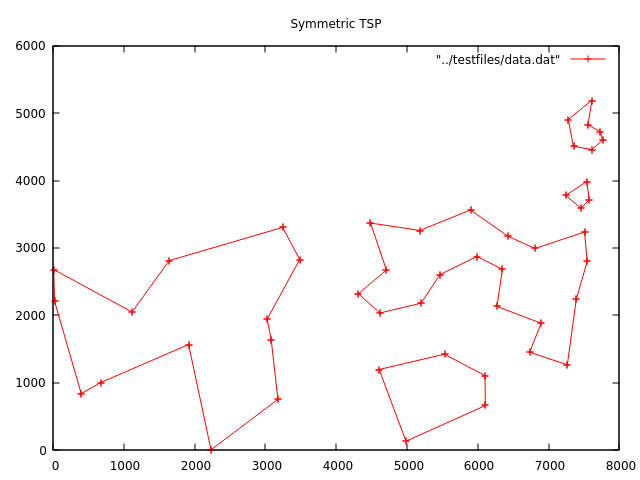
\includegraphics[width=0.6\textwidth]{images/symmetric_with_tours}
	\caption{The image represent att48.tsp solved with the problem formulation showed in section \ref{sec:intro}}
\end{figure}

As we can see the solution that CPLEX found doesn't contain a single tour but a lot of sub-tours. The TSP problem requires that all the nodes must be connected with only one cycle, to do that we implemented different solutions that we will see in this report, the following subsection will explore the basic formulation of the loop method (also known as benders) and some compact models (MTZ and GG).

\subsection{Loop method}
\label{sec:loop}
This method is easier to implement and also easier to understand. This process that we are going to describe is also known as benders decomposition and it is based on the principle of the divide-and-conquer.

%%TODO riscrivere meglio vala'
The basic algorithm is the following: we give CPLEX the same model as before but this time we check if the solution has some sub-tour, if yes then we apply the loop method to each cycle found. Essentially it creates a new constraint and adds it to the problem, the constraint that is going to block the formation of the cycles in the next call of CPLEX. \\
Let's make an example, we have a cycle that is composed by five nodes and consequently by five edges that forms the sub-tour; the constraint we build forces the software to connect those five edges with a maximum of four (number of nodes - $1$) edges, this method must be applied to all the sub-tours found in the solution, then we call again CPLEX to solve the problem. If the problem has again some cycles inside we will apply again the loop method until the nodes are connected with only one cycle.

\begin{figure}[h]
	\centering
	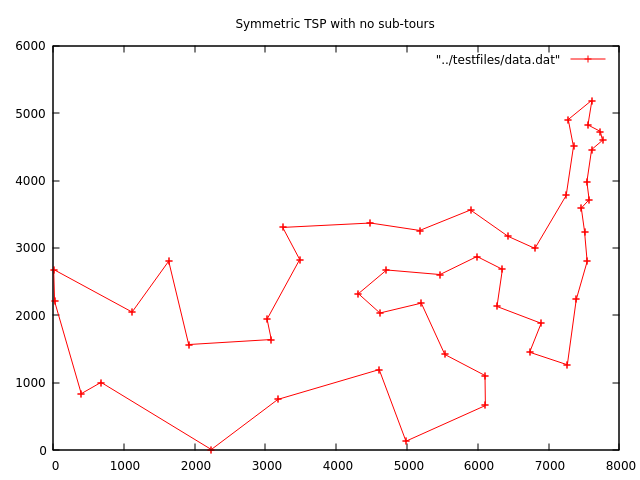
\includegraphics[width=0.6\textwidth]{images/symmetric_with_no_tours}
	\caption{The image represent att48.tsp solved with the loop method described in section \ref{sec:loop}}
\end{figure}

As we can see this time the solution found have no sub-tours and in particular this one was found in circa $0.3$ seconds with a total of 7 iterations where there were added 22 constraints in order to obtain this final solution.

\subsubsection{Particularity of the variable creation in the symmetric TSP}
In the setup section (\ref{cap:2_int}) we have seen how the variable and constraints are implemented inside cplex, we have also seen how we can refer to a variable when using the callable library, by simply using its "position" inside the variable array. It is immediately noticeable that the order in which we create them is really important and allow us to know exactly the position of each variable inside that array.

The way we managed the variables is the following: we think them as they were inside a matrix where the rows are the starting node and the columns are the arriving node. We can see an example in the figure \ref{img:full_matrix}.

\begin{figure}[h]
	\centering
	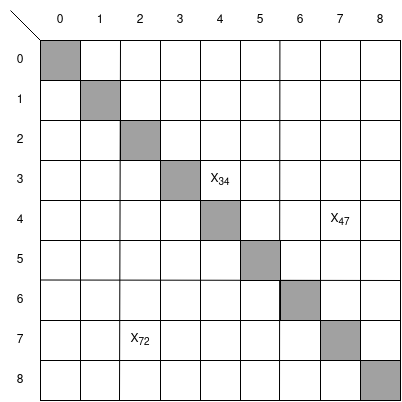
\includegraphics[width=0.55\textwidth]{images/full_matrix}
	\caption{The image represent the matrix method we used to reference the variable inside CPLEX}
	\label{img:full_matrix}
\end{figure}

In this way the is it really simple to find the number of the variable we want to reference, for example if we want to use the index of $x_{34}$ we just need to compute this $3 * (\text{number of nodes}) + 4$ and thats it.

In the particular case of the simmetric TSP the path from $i$ to $j$ and $j$ to $i$ is the same so we don't need all the matrix that we have just showed. So in order to easily obtain the number we image a matrix as the one in the figure \ref{img:full_matrix_simm}, this time all the cells that are in gray are not used since the useful values are saved in the other cells since $x_{ij}$ have the same value than $x_{ji}$.


\begin{figure}[h]
	\centering
	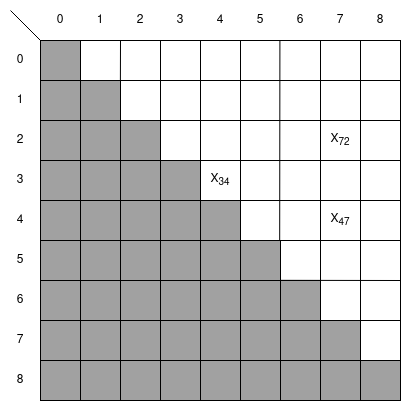
\includegraphics[width=0.55\textwidth]{images/full_matrix_simmetric}
	\caption{The image represent the matrix method we used to reference the variable inside CPLEX in the case of the simmetric TSP. In this case half of the matrix is not used since the values that were in the gray cells are the same of its "corrisponding white cell" since $x_{ij}$ have the same value than $x_{ji}$. In fact the value $x_{72}$ in the figure \ref{img:full_matrix} is transposed into $x_{27}$.}
	\label{img:full_matrix_simm}
\end{figure}

	\section{Resolution with the callback method}
In sectio\ref{sec:problem-resolution} we introduce the fastest resolution method we've seen so far, but its implementation is a little bit tricky, and most of all not really "easthetic" CAMBIARE.\\
In this section we are going to explore the same loop method (so we will reject the solutions with some sub-tours) but this time we will implement its better version, also known as branch and cut.

\subsection{The callbacks}
Let's dive in in the main argument of this section: the callbacks.

As the name can suggest this type of function are not the classical one we have seen in section \ref{sec:setup} and \ref{sec:problem-resolution}, in fact every method of the callable library we have used is applied or before or after the optimization computed by CPLEX. The callback functions give to the user significant additional capabilities because they allow to intervene during the optimization, this upgraded abilities permit the user to work with the internal data structure of CPLEX so the developer must be aware of what he is doing.

CPLEX has three different types of callbacks: informational callbacks, query/diagnostic callbacks, and control callbacks. The first ones gives the user additional information on the current optimization without affection the performance or interfering with the solution search space. The second ones access to more detailed informations respect to the informational callbacks but can affect the overall performance of the problem resolution; the query/diagnostic callbacks are also incompatible with the dynamic search and deterministic parallel functions. The last ones are the one we are going to use and they allow the user to alter and customize how CPLEX perform the optimization.

In order to use them we need to declare their usage before calling the optimization function, we can do this through the function of the callable library:

\begin{lstlisting}
	CPXcallbacksetfunc(env, lp, CPX_CALLBACKCONTEXT_CANDIDATE, sec_callback, inst)
\end{lstlisting}

In this piece of code we can see the variables \verb|env| and \verb|lp| are the well known environment and problem of CPLEX. The third argument (\verb|CPX_CALLBACKCONTEXT_CANDIDATE|) is what the API documentation call contextmask, usually this value must be one of the constants described the callable library; the value passed in the function tells CPLEX to call the callback function (the fourth argument, \verb|sec_callback|) everytime it finds an integer solution of the problem. The last argument is the user data that are passed to the callback function.


\subsection{Callback with an integer solution}
The first callback we analyze are the one that will be called when CPLEX finds an integer solution. Once the function is called we can perform some operations with the informations we can retrieve from the problem. The operations we perform are similar to the ones descripted in section \ref{sec:sol_management}.

First we retrieve the solution found by CPLEX with the function \verb|CPXcallbackgetcandidatepoint|, than we perform the same operations we have done when we described the \verb|build_solution| function, so we find all the components of the solution. When there are more than one componentes, so some sub-tours are present, we add to the problem the reason why the solution is infeasable for us through the function \verb|CPXcallbackrejectcandidate|. The meaning of the function is that the current solution found during the optimization is not feasable since it violetes the costraints that we pass as arguments (in fact are similar to the one used when we used the lazy constraints in the MTZ model).

\subsection{Callback with a fractional solution}
The management of this solutions are really more complex than the one previously analyzed since as all the values in the solution are not integer so we can't handle as we have done before (with the method of the components). Because the operations to perform in order to compute if the solution is composed by sub-tours we decided to use an external static library called \href{https://www.math.uwaterloo.ca/tsp/concorde.html}{Concorde}.
This library is one of the most powerful available in the market, it has even its own iOS application that allow to solve pretty complex instance of the problem.

The problem with this kind of solution its that can contains some nodes where the number of incidence edges is greater that 2 but their values are weighted in such way to respect anyway the degree costraint.

The methods appleid by Concorde to solve the fractional problem require that the graph is connected (using the function \verb|CCcut_connect_components|), if its true we can call another function that allow us to implement the addition of a cut to the problem (performed by \verb|CPXcallbackaddusercuts|).

\subsection{Performance Analysis}
SCIRVERE QUI LE PERFEORMANCE

%Spiegare il funzionamento 
	\section{Heuristics}
\label{sec:heuristics}
Sometimes the complexity of the problem is too much to be solved by a machine (either for its power or the problem complexity). In that conditions we decided to renounce to obtain the optimal solution in favor of a fast solution, even if it is suboptimal.

The algorimths that implement this concept are called heuristics and their strategies are as simple as they are quick. \\
We are going to explore some of this heuristics, in particular:
\begin{itemize}
	\item greedy;
	\item extra-mileage;
	\item k-opt;
	\item variable neighboorhood search.
\end{itemize}

\subsection{Greedy algorithm}
The greedy algorithm is the easiest to understand. It starts from a random node and than it execute a greedy choice by choosing the arc with the lower cost between the ones that are not connect to a node that is already in the solution. The algorithm performs this operation until all the nodes are in the solution.

This simple idea as a negative effect, in fact the algorithm prefers the nodes that are close to each other and leaves alone the node that are more distant; since all the nodes must be in the solution even the fartest node needs to be chosen at some point, by delaying their choice the greedy method is forced to connect theese nodes provoking the usage of really long edges that surely are not in the optimal solution.

In our code we decide to perform a particular implementation, we start execution the algorithm starting from each node and than we choose the best solution found through the iterations. The problem with this approach is that we slow down the procedd by a factor $n$ because we need to search the best solution among all the nodes used as start.

\begin{figure}
	\label{img:greedy}
	\centering
	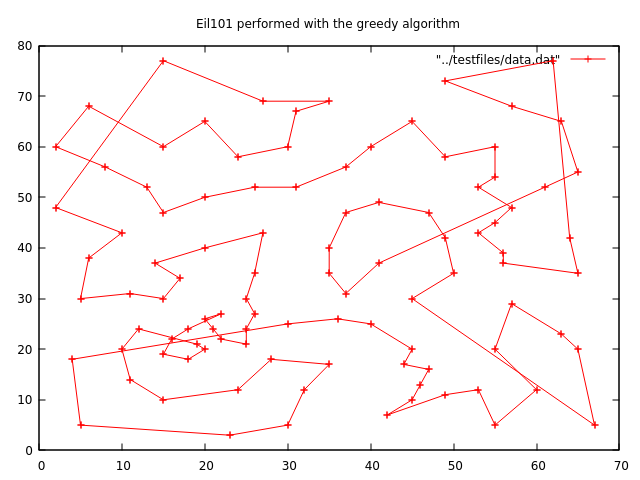
\includegraphics[width=0.6\textwidth]{images/eil101_greedy}
	\caption{In this figure we can see the application to eil101.tsp of the greedy algorithm. In particular we can see the long edges that are chosen since the procedure prefers the nodes that are close to each other.}
\end{figure}

\subsection{Extra-mileage algorithm}
This algorithm is more complex respect to the previous one but in favor of a better solution.

The idea in which the extra-mileage is the following: we start connecting the fartest nodes with both edges (like a cycle), than we search for the closest node to the edges, once it has been identified the edge is substitute with a new couple that insert the the node found in the solution. Let's explain it with the example shown in figure \ref{img:extra}.

\begin{figure}
	\centering
	\begin{subfigure}[b]{0.3\textwidth}
		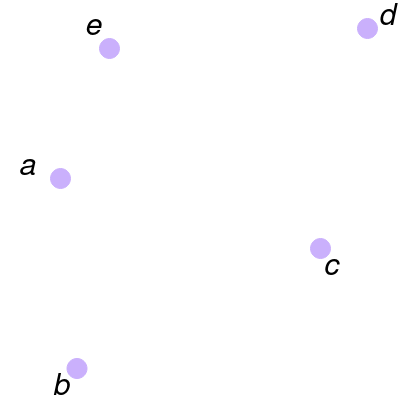
\includegraphics[width=\textwidth]{images/extra_1}
		\caption{No edges}
	\end{subfigure}
	\hfill
	\begin{subfigure}[b]{0.3\textwidth}
		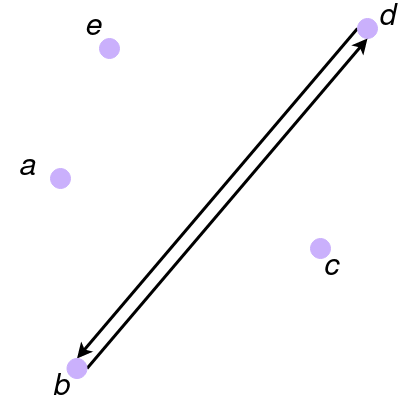
\includegraphics[width=\textwidth]{images/extra_2}
		\caption{First two edges added}
	\end{subfigure}
	\hfill
	\begin{subfigure}[b]{0.3\textwidth}
		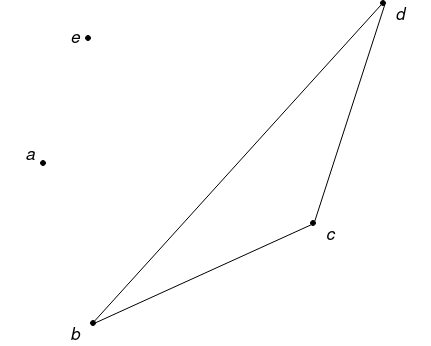
\includegraphics[width=\textwidth]{images/extra_3}
		\caption{One edge is substituted with other two connecting one more node}
	\end{subfigure}
	\bigskip
	\begin{subfigure}{0.3\textwidth}
		\centering
		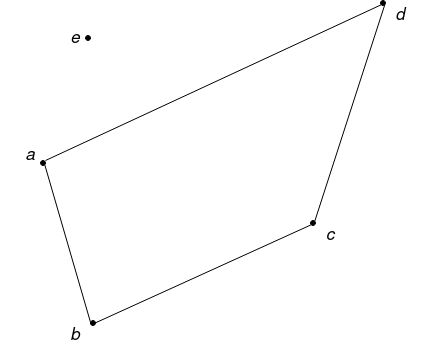
\includegraphics[width=\textwidth]{images/extra_4}
		\caption{Added one more node}
	\end{subfigure}
	\hfill
	\begin{subfigure}{0.3\textwidth}
		\centering
		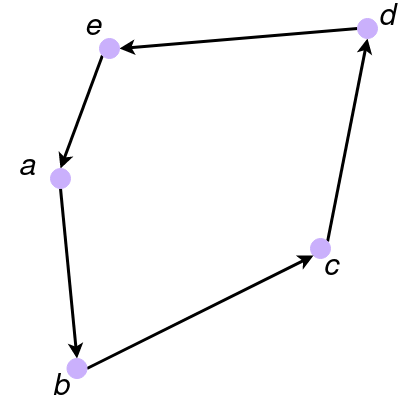
\includegraphics[width=\textwidth]{images/extra_5}
		\caption{All nodes are connected}
	\end{subfigure}
	\caption{In this image we can see the process done by extra-mileage to find the solution.}
	\label{img:extra}
\end{figure}

We start connecting with a cycle the fartest nodes (in this case $c$ and $d$), than we search the node that is closest to theese edges ($c$), once is found we substitute the edge with two more that allow the new node to enter the solution (in this case in order to allow $c$ to enter the solution one of the edges that connect $b$ and $c$ is removed and the edge $x_{bc}$ and $x_{cd}$ are added). This process is repeated until the solution is formed.

We can see the result of the algorithm in figure \ref{img:extra_sol}. Respect to the greedy algorithm we can see that is more ordered with less crossed edges.

\begin{figure}
	\centering
	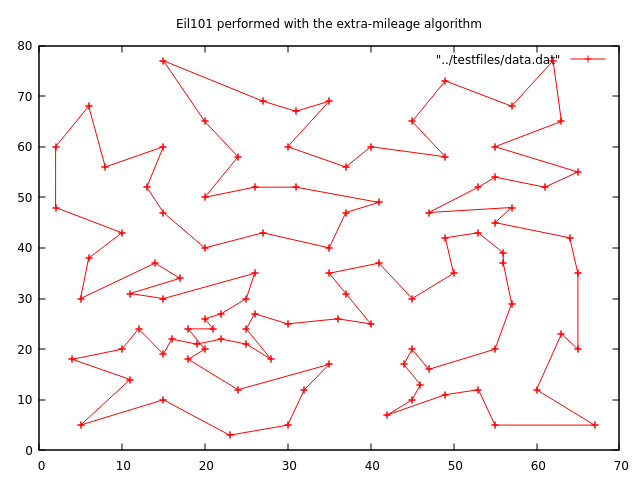
\includegraphics[width=0.6\textwidth]{images/eil101_extra_mileage}
	\caption{In this figure we can see the result of the application of the extra-mileage algortihm to eil101.tsp}
	\label{img:extra_sol}
\end{figure}

\subsection{k-\textit{opt} refining}
This section is not about an algorithm to solve the TSP problem but is about to refine (so improve) a solution that is already been found.\\
The process is based on the triangle inequality, in fact we are going to remove all the edges that cross each other. We can see an example of this operation in the image \ref{img:k_opt_example}, where the two edges that cross each other are sostitute by other to edges.

From a theoretical point of view the k-opt operation is a local search on the current solution, is not guaranteed to reach an optimal solution, but the objective value of the solution is going to always improve (if possible), in the worst case the solution will not change.

In our case we implemented two k-opt algorithms, the 2-opt and the 3-opt. We have decided to do that since as the $k$ grows the complexity grows with it. Just the implementation of the 3-opt algorithm is quite expensive from a computational point of view.

In the figure \ref{img:k_opt} we can see the differences between the 2-opt and 3-opt refining. In this images we applied theese algorithms starting from the solution provided by the greedy method to kroA200.tsp. \\
In the 2-opt application we started from a solution cost of $34543.0$ and than by the refining algorithm we reached the value $30189.0$ with a very little computational time, in fact it needed only $0.65$ seconds to reach the final solution.\\
In the 3-opt application we started from a solution cost of $34543.0$ and than by the refining algorithm we reached the value $25379.0$ in $77.37$ seconds.\\


\begin{figure}
	
	\centering
	\begin{subfigure}[b]{0.5\textwidth}
		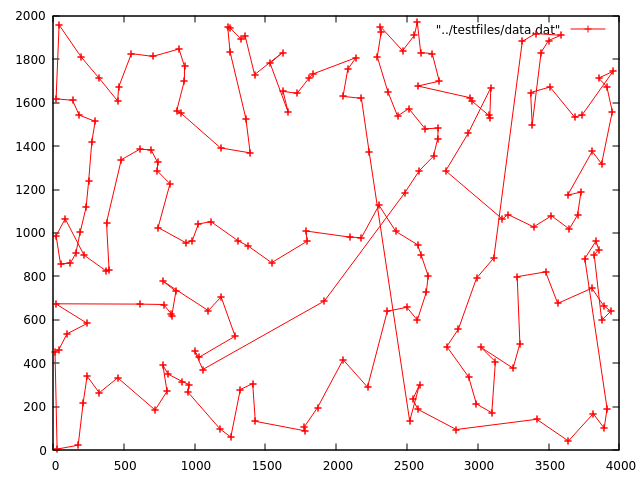
\includegraphics[width=\textwidth]{images/kroA_greedy}
		\caption{The instance kroA200.tsp solved with the greedy algorithm}
	\end{subfigure}
	\bigskip
	\begin{subfigure}[b]{0.5\textwidth}
		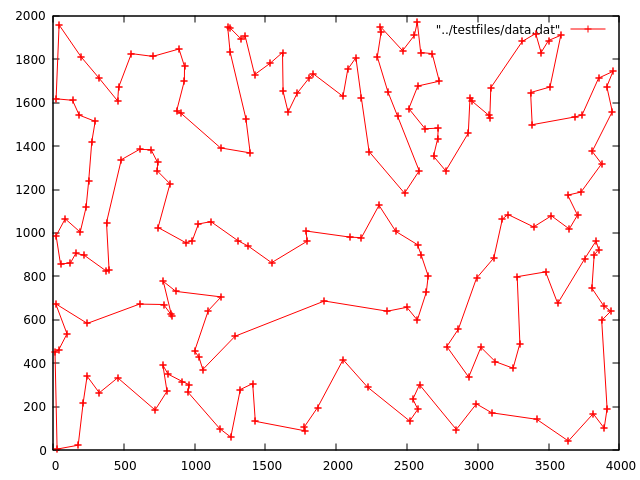
\includegraphics[width=\textwidth]{images/2_opt}
		\caption{Greedy + 2-opt refining}
	\end{subfigure}
	\bigskip
	\begin{subfigure}[b]{0.5\textwidth}
		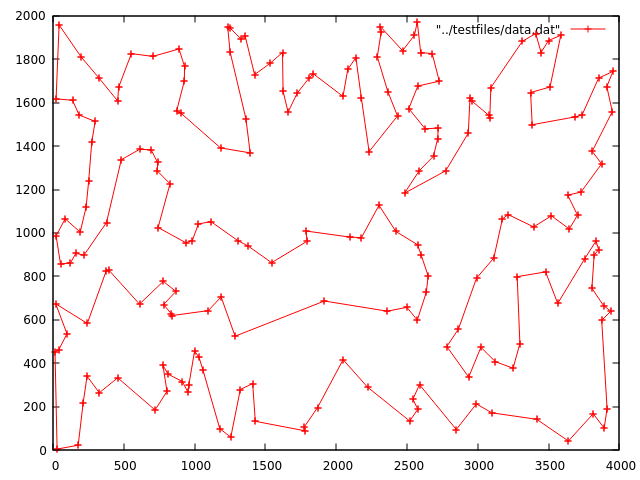
\includegraphics[width=\textwidth]{images/3_opt}
		\caption{Greedy + 3-opt refining}
	\end{subfigure}
	\caption{Comparison between the 2-opt and 3-opt refining}
	\label{img:k_opt}
\end{figure}

\subsection{Heuristics based on the branch and cut}
This section will explore the application of two heuristrics in the branch and cut method that we have seen in section \ref{sec:branch_and_cut}. Using these methods we can allow to the branch and cut method to solve even big instances but in a way that they probably never reach the optimal solution. The starting point of this section is basically the reduction of the search space.


\subsubsection{Hard-fixing}
The method of the hard-fixing expect to block the value of some variables in the problem in order to get the search space reduce in order to compute more easily a solution for it. The choice of which variable to block is due the user, but eventually can be completely random. 

The most important setting for this method is the starting solution, in fact since we are blocking the varibles so if the satarting solution is completely wrong the process of improving it will be more difficult. The process to retrieve a final solution is pretty easy: we start from that solution, we apply the branch and cut method for a predermined amount of time (or until it finds the optimal solution in the seach subspace), at the end of it we check if the new solution found is actually better than the previous one, if not we reduce the number of blocked variables and repeat the process. 

In our implementation we decided to put a percentage on the number of blocked variables, in particular we started from a value of $90\%$ and than for each time the solution found was not better than the previous one we reduced it by a $20\%$. The solution chosen as start was simply computed by the branch and cut method with the same time limit setted in the algorithm, in this way the starting point should never be a worse one.


\subsubsection{Soft-fixing}
	%\bibliography{bibliography}
\end{document}